% !TEX encoding = UTF-8
% !TEX TS-program = pdflatex
% !TEX root = ../tesi.tex

%**************************************************************
\chapter{Analisi comparativa dei protocolli REST e GraphQL}
\label{cap:analisi-comparativa}
%**************************************************************
\intro{In questo capitolo verrà svolta l'analisi comparativa tra i due protocolli REST e GraphQL, sia dal punto di vista teorico che da quello pratico .}\\
%**************************************************************
%\section{Analisi comparativa teorica}
%\label{sec:analisi-comparativa-teorica}
%Per analisi comparativa teoria s'intende tutti quegli aspetti che differenziano i due protocolli GraphQL e REST
\section{Introduzione}
REST è stato ed è tutt'oggi lo standard più seguito per la realizzazione delle Web API, tuttavia dopo l'uscita di GraphQL il suo monopolio è stato messo in crisi. Infatti GraphQL ha portato con se delle interessanti soluzioni per molti dei problemi e dei vincoli dello stile architetturale REST.\\
L'innovazione portata da GraphQL è stata apprezzata in larga scala tra gli sviluppatori, a conferma di ciò è possibile visualizzare nell'immagine \ref{graphQL-usage-chart} l'aumento nell'utilizzo di questa tecnologia con il passare degli anni.
\FloatBarrier
\begin{figure}[!ht]
\centering
\includegraphics[width=1\linewidth]{immagini/GraphQLUsageChart.png}
\caption{Grafico sull'utilizzo di GraphQL negli anni.}
\label{graphQL-usage-chart}
\end{figure}
\FloatBarrier
Nel seguente capitolo verranno analizzati nel dettaglio e paragonati i due protocolli, sotto tutti i punti di vista, mettendo in risalto vantaggi e svantaggi di ciascuno; infine verranno riportate le deduzioni elaborate durante lo stage sul protocollo che è meglio seguire in base all'applicativo che si vuole sviluppare.
\section{Analisi comparativa}
Come sottolineato in precedenza, GraphQL e REST hanno diversi aspetti che li differenziano. La più grande differenza tra questi due protocolli è legata alla loro natura: infatti quando si fa riferimento a REST, si sta parlando di uno stile architetturale, dunque di un modo di costruire le proprie API le quali, se rispettano i vincoli REST illustrati al punto \ref{principi-REST}, vengono definite RESTful. Quando si fa riferimento a GraphQL invece, si sta parlando di un linguaggio di query fortemente tipizzato.\\\\
Di seguito è presente un'analisi comparativa dettagliata per ciascun aspetto che differenzia i due protocolli di data fetching.
\subsection{Endpoints}
La prima grossa differenza tra i due protocolli riguarda gli endpoint.\\
Lo stile REST prevede l'utilizzo di più endpoint, sfrutta infatti la molteplicità degli endpoint per differenziare le richieste possibili. Quando un client implementa una richiesta a delle REST API deve sapere esattamente a quale endpoint inviare la richiesta per ricevere i dati necessari. In figura \ref{REST-endpoints} viene rappresentato un REST server che fornisce diversi endpoint e il client, il quale invia diverse richieste a diversi endpoint.
\FloatBarrier
\begin{figure}[!ht]
\centering
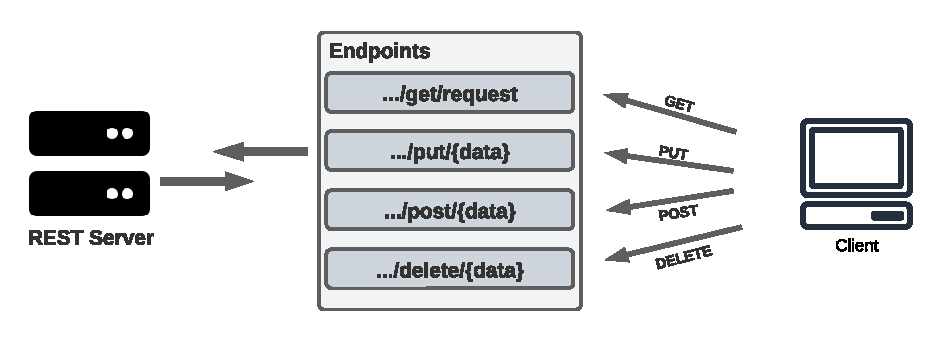
\includegraphics[width=1\linewidth]{immagini/RESTEndpoints.pdf}
\caption{Gli endpoints multipli in REST.}
\label{graphQL-usage-chart}
\end{figure}
\FloatBarrier
Con GraphQL questo non avviene, infatti GraphQL prevede l'esposizione di un unico endpoint. A questo singolo endpoint possono essere inviate tutte le richieste inserendo nel body della richiesta la query, la mutation o la subscription. In figura \ref{GraphQL-endpoint} è possibile visualizzare come il GraphQL server fornisca un unico endpoint e come il client invii tutti i tipi di richieste allo stesso medesimo endpoint.
\FloatBarrier
\begin{figure}[!ht]
\centering
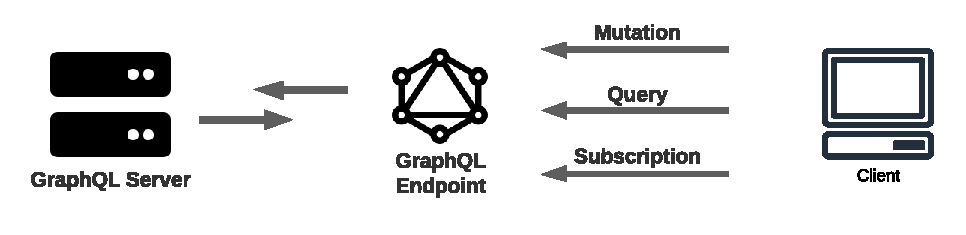
\includegraphics[width=1\linewidth]{immagini/GraphQLEndpoint.pdf}
\caption{Il singolo endpoint GraphQL.}
\label{GraphQL-endpoint}
\end{figure}
\FloatBarrier
A proposito di ciò viene riportata di seguito una citazione di Lee Byron, il co-creatore di GraphQL:
\begin{quoting}
  \textit{"Think in graphs, not endpoints."}
\end{quoting}
\subsection{Overfetching e Underfetching}
La questione dell'overfetching e underfetching è uno degli aspetti che viene maggiormente considerato nella decisione architetturale riguardo quale protocollo di data fetching utilizzare tra REST e GraphQL.\\
Lo stile architetturale REST non prevede di definire lato client esattamente quali dati ricevere. Un client che necessita un certo insieme da un server con REST API, è costretto ad eseguire una o più richieste e dunque a prendersi in carico della rielaborazione dei dati. Per uno sviluppatore backend è molto complesso riuscire a creare delle REST API che siano in grado di soddisfare esattamente le tutte le richieste dei client.
L'introduzione di GraphQL come nuovo protocollo di data fetching ha posto una soluzione a questo problema, permettendo al client di specificare esattamente la forma e il quantitativo di dati necessari. Quando si decide di implementare un applicativo e si valuta quale protocollo di data fetching utilizzare, questo è sicuramente un punto da considerare.\\
\paragraph{Overfetching}
Quando si parla di overfetching si fa riferimento al fatto che vengano forniti più dati di quanti realmente necessari. Riprendendo come esempio il prototipo visto nel capitolo \ref{casi-uso}, si suppone che il client necessiti della lista degli impiegati e che, per ciascun impiegato, necessiti  esclusivamente l'id e il nome. Qualora si tratti della version REST del server, il client inviare la richiesta HTTP all'endpoint mappato sul metodo \textit{allEmployee()}, il quale ritorna una lista di impiegati e, per ciascun impiegato, tutti i campi. Di seguito il JSON di risposta che il client riceve in seguito alla richiesta nel caso in cui fossero presenti solo due impiegati:
\begin{verbatim}
  [
    {
        "id": "3AFASDF12F",
        "name": "Matteo",
        "surname": "Verdi",
        "salary": 1500,
        "birth": "1995-02-21"
    },
    {
        "id": "GA14PL3FAV",
        "name": "Marco",
        "surname": "Blu",
        "salary": 1500,
        "birth": "1993-12-20"
    }
  ]
\end{verbatim}
Si può subito notare come i campi \textit{surname}, \textit{salary} e \textit{birth} non siano necessari in quanto il client utilizza solo i campi \textit{id} e \textit{name}. Nel caso del prototipo si tratta di un problema irrisorio data la ridotta grandezza dei dati, tuttavia in applicativi a larga scala che richiedono grossi quantitativi di dati complessi può risultare un problema in termini di occupazione di rete e di rallentamenti dell'applicativo. Questo problema può essere risolto in un server con REST API fornendo endpoint specifici per ciascun tipo di richiesta, tuttavia questa soluzione rischia di introdurre confusione e nel tempo la manutenzione potrebbe risultare sempre più complessa.\\
GraphQL risolve questo problema attribuendo al client la responsabilità di definire quali siano i campi di cui necessita. Questo è possibile specificando nella query i campi richiesti, di seguito l'esempio dell'invocazione contenente a sinistra la query \textit{allEmployee}, mentre a destra il JSON ricevuto in risposta:
\begin{verbatim}
    QUERY                                     JSON RETURNED

    query getAllEmployee{                 [
      allEmployee {                         {
        Employee {                              "id": "3AFASDF12F",
          id                                    "name": "Matteo"
          name                              },
          }                                 {
      }                                          "id": "GA14PL3FAV",
    }                                            "name": "Marco"
                                            }
                                          ]
\end{verbatim}
In GraphQL questo approcio permette di non sovraccaricare inutilmente la rete e di mantenere ordinato e di facile manutenzione la struttura API del server. Lato client è richiesto un maggior sforzo per nella specifica della query, ma d'altra parte si evitano problemi di rallentamento o errori dovuti al fetching di grossi quantitativi di dati inutili. 
\section{Conclusioni}





% Spiegazione di cosa si intende per analisi comparativa teorica: analisi % comparativa che va a comparare gli aspetti prettamente teorici, come ad esempio:
% \begin{itemize}
%  \item overfetching e underfetching;
%  \item un protocollo è una sorta di standard/stile architetturale (restfull api)     mentre l'altro un linguaggio di query fortemente tipizzato (REST invece non è safe dal punto di vista dei tipi);
%  \item come sfruttano il protocollo http (stati risposte http, endpoint multipli vs singolo, ecc...);
%  \item manuntenibilità nel tempo;
%  \item documentazione (GraphQL si autodocumenta, REST no);
%  \item meccanismo di caching integrato (mancante in GraphQL);
%  \item formati output di risposta (GraphQL --> JSON, REST --> JSON, XML, YAML);
% \end{itemize}
% \section{Analisi comparativa sui casi d'uso}
% Analisi comparativa basata su:
% \begin{itemize}
%  \item differenze nell'analisi e progettazione iniziale delle API;
%  \item differenze durante lo sviluppo delle API dal punto di vista di BE e FE(anche legate agli strumenti utilizzati ad es. Spring Data REST vs Spring GraphQL);
%  \item differenze prestazionali (utilizzato tool K6 per load test);
% \end{itemize}2
